\documentclass{article}
% translate with >> pdflatex -shell-escape <file>

% This file is an extract of the PGFPLOTS manual, copyright by Christian Feuersaenger.
% 
% Feel free to use it as long as you cite the pgfplots manual properly.
%
% See
%   http://pgfplots.sourceforge.net/pgfplots.pdf
% for the complete manual.
%
% Any required input files (for <plot table> or <plot file> or the table package) can be downloaded
% at
% http://www.ctan.org/tex-archive/graphics/pgf/contrib/pgfplots/doc/latex/
% and
% http://www.ctan.org/tex-archive/graphics/pgf/contrib/pgfplots/doc/latex/plotdata/

\usepackage{pgfplots}
\pgfplotsset{compat=newest}

\pagestyle{empty}

\usepgfplotslibrary{patchplots}

\begin{document}
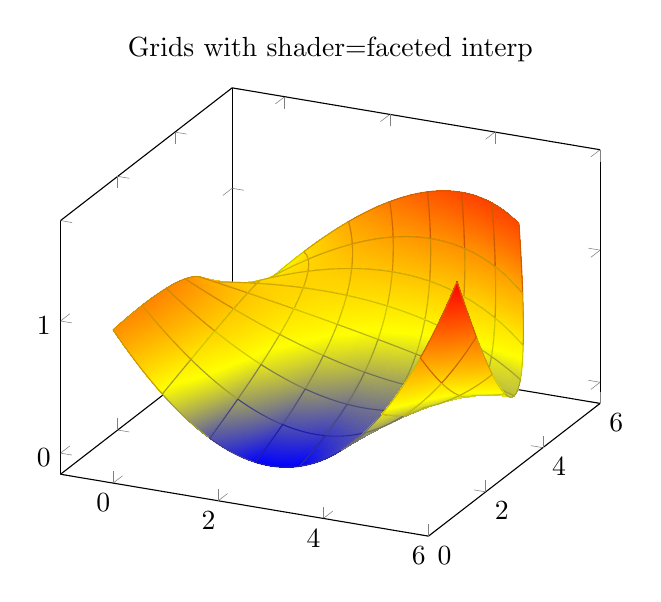
\begin{tikzpicture}
\begin{axis}[
	title={Grids with shader=faceted interp}]

\addplot3[patch,patch type=biquadratic,
	shader=faceted interp,patch refines=3]
coordinates {
	(0,0,1) (6,1,1.6) (5,5,1.3) (-1,5,0)
	(3,1,0) (6,3,0.4) (2,6,1.1) (0,3,0.9)
	(3,3.75,0.5)
};
\end{axis}
\end{tikzpicture}
\end{document}
